\documentclass[12pt,landscape]{article}

%\usepackage{lmodern}
\usepackage{amssymb,amsmath}
\usepackage{bm}
\usepackage{graphicx}
\usepackage{microtype}
\usepackage{hyperref}
\pagestyle{empty}
\usepackage{titlesec}
\titleformat*{\section}{\LARGE\bfseries}
\titleformat*{\subsection}{\LARGE\bfseries}
\titleformat*{\subsubsection}{\LARGE\bfseries}
\setlength{\parindent}{0pt}
\setlength{\parskip}{1.2ex}
\setlength{\parindent}{0pt}
\setlength{\parskip}{1.2ex}

\setlength{\oddsidemargin}{-16mm}
\setlength{\textwidth}{260mm}
\setlength{\columnsep}{0.5in}
\setlength{\columnseprule}{1pt}
\setlength{\textheight}{202mm}
\setlength{\topmargin}{-32mm}
\setlength{\headsep}{0.25in}

\hypersetup
       {   pdfauthor = { Marco Fasondini },
           pdftitle={ foo },
           colorlinks=TRUE,
           linkcolor=black,
           citecolor=blue,
           urlcolor=blue
       }




\usepackage{upquote}
\usepackage{listings}
\usepackage{xcolor}
\lstset{
    basicstyle=\ttfamily\footnotesize,
    upquote=true,
    breaklines=true,
    breakindent=0pt,
    keepspaces=true,
    showspaces=false,
    columns=fullflexible,
    showtabs=false,
    showstringspaces=false,
    escapeinside={(*@}{@*)},
    extendedchars=true,
}
\newcommand{\HLJLt}[1]{#1}
\newcommand{\HLJLw}[1]{#1}
\newcommand{\HLJLe}[1]{#1}
\newcommand{\HLJLeB}[1]{#1}
\newcommand{\HLJLo}[1]{#1}
\newcommand{\HLJLk}[1]{\textcolor[RGB]{148,91,176}{\textbf{#1}}}
\newcommand{\HLJLkc}[1]{\textcolor[RGB]{59,151,46}{\textit{#1}}}
\newcommand{\HLJLkd}[1]{\textcolor[RGB]{214,102,97}{\textit{#1}}}
\newcommand{\HLJLkn}[1]{\textcolor[RGB]{148,91,176}{\textbf{#1}}}
\newcommand{\HLJLkp}[1]{\textcolor[RGB]{148,91,176}{\textbf{#1}}}
\newcommand{\HLJLkr}[1]{\textcolor[RGB]{148,91,176}{\textbf{#1}}}
\newcommand{\HLJLkt}[1]{\textcolor[RGB]{148,91,176}{\textbf{#1}}}
\newcommand{\HLJLn}[1]{#1}
\newcommand{\HLJLna}[1]{#1}
\newcommand{\HLJLnb}[1]{#1}
\newcommand{\HLJLnbp}[1]{#1}
\newcommand{\HLJLnc}[1]{#1}
\newcommand{\HLJLncB}[1]{#1}
\newcommand{\HLJLnd}[1]{\textcolor[RGB]{214,102,97}{#1}}
\newcommand{\HLJLne}[1]{#1}
\newcommand{\HLJLneB}[1]{#1}
\newcommand{\HLJLnf}[1]{\textcolor[RGB]{66,102,213}{#1}}
\newcommand{\HLJLnfm}[1]{\textcolor[RGB]{66,102,213}{#1}}
\newcommand{\HLJLnp}[1]{#1}
\newcommand{\HLJLnl}[1]{#1}
\newcommand{\HLJLnn}[1]{#1}
\newcommand{\HLJLno}[1]{#1}
\newcommand{\HLJLnt}[1]{#1}
\newcommand{\HLJLnv}[1]{#1}
\newcommand{\HLJLnvc}[1]{#1}
\newcommand{\HLJLnvg}[1]{#1}
\newcommand{\HLJLnvi}[1]{#1}
\newcommand{\HLJLnvm}[1]{#1}
\newcommand{\HLJLl}[1]{#1}
\newcommand{\HLJLld}[1]{\textcolor[RGB]{148,91,176}{\textit{#1}}}
\newcommand{\HLJLs}[1]{\textcolor[RGB]{201,61,57}{#1}}
\newcommand{\HLJLsa}[1]{\textcolor[RGB]{201,61,57}{#1}}
\newcommand{\HLJLsb}[1]{\textcolor[RGB]{201,61,57}{#1}}
\newcommand{\HLJLsc}[1]{\textcolor[RGB]{201,61,57}{#1}}
\newcommand{\HLJLsd}[1]{\textcolor[RGB]{201,61,57}{#1}}
\newcommand{\HLJLsdB}[1]{\textcolor[RGB]{201,61,57}{#1}}
\newcommand{\HLJLsdC}[1]{\textcolor[RGB]{201,61,57}{#1}}
\newcommand{\HLJLse}[1]{\textcolor[RGB]{59,151,46}{#1}}
\newcommand{\HLJLsh}[1]{\textcolor[RGB]{201,61,57}{#1}}
\newcommand{\HLJLsi}[1]{#1}
\newcommand{\HLJLso}[1]{\textcolor[RGB]{201,61,57}{#1}}
\newcommand{\HLJLsr}[1]{\textcolor[RGB]{201,61,57}{#1}}
\newcommand{\HLJLss}[1]{\textcolor[RGB]{201,61,57}{#1}}
\newcommand{\HLJLssB}[1]{\textcolor[RGB]{201,61,57}{#1}}
\newcommand{\HLJLnB}[1]{\textcolor[RGB]{59,151,46}{#1}}
\newcommand{\HLJLnbB}[1]{\textcolor[RGB]{59,151,46}{#1}}
\newcommand{\HLJLnfB}[1]{\textcolor[RGB]{59,151,46}{#1}}
\newcommand{\HLJLnh}[1]{\textcolor[RGB]{59,151,46}{#1}}
\newcommand{\HLJLni}[1]{\textcolor[RGB]{59,151,46}{#1}}
\newcommand{\HLJLnil}[1]{\textcolor[RGB]{59,151,46}{#1}}
\newcommand{\HLJLnoB}[1]{\textcolor[RGB]{59,151,46}{#1}}
\newcommand{\HLJLoB}[1]{\textcolor[RGB]{102,102,102}{\textbf{#1}}}
\newcommand{\HLJLow}[1]{\textcolor[RGB]{102,102,102}{\textbf{#1}}}
\newcommand{\HLJLp}[1]{#1}
\newcommand{\HLJLc}[1]{\textcolor[RGB]{153,153,119}{\textit{#1}}}
\newcommand{\HLJLch}[1]{\textcolor[RGB]{153,153,119}{\textit{#1}}}
\newcommand{\HLJLcm}[1]{\textcolor[RGB]{153,153,119}{\textit{#1}}}
\newcommand{\HLJLcp}[1]{\textcolor[RGB]{153,153,119}{\textit{#1}}}
\newcommand{\HLJLcpB}[1]{\textcolor[RGB]{153,153,119}{\textit{#1}}}
\newcommand{\HLJLcs}[1]{\textcolor[RGB]{153,153,119}{\textit{#1}}}
\newcommand{\HLJLcsB}[1]{\textcolor[RGB]{153,153,119}{\textit{#1}}}
\newcommand{\HLJLg}[1]{#1}
\newcommand{\HLJLgd}[1]{#1}
\newcommand{\HLJLge}[1]{#1}
\newcommand{\HLJLgeB}[1]{#1}
\newcommand{\HLJLgh}[1]{#1}
\newcommand{\HLJLgi}[1]{#1}
\newcommand{\HLJLgo}[1]{#1}
\newcommand{\HLJLgp}[1]{#1}
\newcommand{\HLJLgs}[1]{#1}
\newcommand{\HLJLgsB}[1]{#1}
\newcommand{\HLJLgt}[1]{#1}



\def\qqand{\qquad\hbox{and}\qquad}
\def\qqfor{\qquad\hbox{for}\qquad}
\def\qqas{\qquad\hbox{as}\qquad}
\def\half{ {1 \over 2} }
\def\D{ {\rm d} }
\def\I{ {\rm i} }
\def\E{ {\rm e} }
\def\C{ {\mathbb C} }
\def\R{ {\mathbb R} }
\def\H{ {\mathbb H} }
\def\Z{ {\mathbb Z} }
\def\CC{ {\cal C} }
\def\FF{ {\cal F} }
\def\HH{ {\cal H} }
\def\LL{ {\cal L} }
\def\vc#1{ {\mathbf #1} }
\def\bbC{ {\mathbb C} }



\def\fR{ f_{\rm R} }
\def\fL{ f_{\rm L} }

\def\qqqquad{\qquad\qquad}
\def\qqwhere{\qquad\hbox{where}\qquad}
\def\Res_#1{\underset{#1}{\rm Res}\,}
\def\sech{ {\rm sech}\, }
\def\acos{ {\rm acos}\, }
\def\asin{ {\rm asin}\, }
\def\atan{ {\rm atan}\, }
\def\Ei{ {\rm Ei}\, }
\def\upepsilon{\varepsilon}


\def\Xint#1{ \mathchoice
   {\XXint\displaystyle\textstyle{#1} }%
   {\XXint\textstyle\scriptstyle{#1} }%
   {\XXint\scriptstyle\scriptscriptstyle{#1} }%
   {\XXint\scriptscriptstyle\scriptscriptstyle{#1} }%
   \!\int}
\def\XXint#1#2#3{ {\setbox0=\hbox{$#1{#2#3}{\int}$}
     \vcenter{\hbox{$#2#3$}}\kern-.5\wd0} }
\def\ddashint{\Xint=}
\def\dashint{\Xint-}
% \def\dashint
\def\infdashint{\dashint_{-\infty}^\infty}




\def\addtab#1={#1\;&=}
\def\ccr{\\\addtab}
\def\ip<#1>{\left\langle{#1}\right\rangle}
\def\dx{\D x}
\def\dt{\D t}
\def\dz{\D z}
\def\ds{\D s}

\def\rR{ {\rm R} }
\def\rL{ {\rm L} }

\def\norm#1{\left\| #1 \right\|}

\def\pr(#1){\left({#1}\right)}
\def\br[#1]{\left[{#1}\right]}

\def\abs#1{\left|{#1}\right|}
\def\fpr(#1){\!\pr({#1})}

\def\sopmatrix#1{ \begin{pmatrix}#1\end{pmatrix} }

\def\endash{–}
\def\emdash{—}
\def\mdblksquare{\blacksquare}
\def\lgblksquare{\blacksquare}
\def\scre{\E}
\def\mapengine#1,#2.{\mapfunction{#1}\ifx\void#2\else\mapengine #2.\fi }

\def\map[#1]{\mapengine #1,\void.}

\def\mapenginesep_#1#2,#3.{\mapfunction{#2}\ifx\void#3\else#1\mapengine #3.\fi }

\def\mapsep_#1[#2]{\mapenginesep_{#1}#2,\void.}


\def\vcbr[#1]{\pr(#1)}


\def\bvect[#1,#2]{
{
\def\dots{\cdots}
\def\mapfunction##1{\ | \  ##1}
	\sopmatrix{
		 \,#1\map[#2]\,
	}
}
}



\def\vect[#1]{
{\def\dots{\ldots}
	\vcbr[{#1}]
} }

\def\vectt[#1]{
{\def\dots{\ldots}
	\vect[{#1}]^{\top}
} }

\def\Vectt[#1]{
{
\def\mapfunction##1{##1 \cr}
\def\dots{\vdots}
	\begin{pmatrix}
		\map[#1]
	\end{pmatrix}
} }

\def\addtab#1={#1\;&=}
\def\ccr{\\\addtab}

\def\questionequals{= \!\!\!\!\!\!{\scriptstyle ? \atop }\,\,\,}

\def\cent#1{\begin{center}#1\end{center} }

\def\Ei{\rm Ei\,}

\lstset{
    basicstyle=\ttfamily,
	}

\begin{document}
{\LARGE
\sf
\textbf{Applied Complex Analysis}

\section{Solution Sheet 4}
\subsection{Problem 1}
\subsubsection{Problem 1.1}
Since $\int_{-1}^1 x \dx = 0$, we have no logarithmic growth at infinity. Thus by the formula relating log to Cauchy transforms we find for

\[
F(x) = \int_x^1 t \dt = {1 - x^2 \over 2}
\]
that

\[
\int_{-1}^1 \log|z-x| x \dx = \Re\pr({2 \I \pi \CC F(z)})
\]
So we just have to work out the Cauchy transform. Try as an ansatz

\[
{1 - z^2 \over 2} {\log(z-1) - \log(z+1) \over 2 \pi \I}
\]
We only need to remove the growth at infinity. We do so via:

\[
\log(z-1) - \log(z+1)  = -{2 \over z} + O(z^{-3})
\]
telling us

\[
\CC F(z) = {1 - z^2 \over 2} {\log(z-1) - \log(z+1)  \over 2 \pi \I} - {z \over 2 \pi \I}
\]
and

\[
\int_{-1}^1 \log|z-x| x \dx = \Re \left({1 - z^2 \over 2} (\log(z-1) - \log(z+1)) - z \right)
\]
\emph{Verification}

We can confirm the formula:


\begin{lstlisting}
(*@\HLJLk{using}@*) (*@\HLJLn{ApproxFun}@*)(*@\HLJLp{,}@*) (*@\HLJLn{SingularIntegralEquations}@*)(*@\HLJLp{,}@*) (*@\HLJLn{Plots}@*)(*@\HLJLp{,}@*) (*@\HLJLn{QuadGK}@*)(*@\HLJLp{,}@*) (*@\HLJLn{LinearAlgebra}@*)(*@\HLJLp{,}@*) (*@\HLJLn{SpecialFunctions}@*)
(*@\HLJLk{import}@*) (*@\HLJLn{ApproxFunOrthogonalPolynomials}@*)(*@\HLJLoB{:}@*) (*@\HLJLn{Recurrence}@*)

(*@\HLJLnf{H}@*)(*@\HLJLp{(}@*)(*@\HLJLn{f}@*)(*@\HLJLp{,}@*)(*@\HLJLn{x}@*)(*@\HLJLp{)}@*) (*@\HLJLoB{=}@*) (*@\HLJLoB{-}@*)(*@\HLJLnf{hilbert}@*)(*@\HLJLp{(}@*)(*@\HLJLn{f}@*)(*@\HLJLp{,}@*)(*@\HLJLn{x}@*)(*@\HLJLp{)}@*)
(*@\HLJLnf{H}@*)(*@\HLJLp{(}@*)(*@\HLJLn{f}@*)(*@\HLJLp{)}@*) (*@\HLJLoB{=}@*) (*@\HLJLoB{-}@*)(*@\HLJLnf{hilbert}@*)(*@\HLJLp{(}@*)(*@\HLJLn{f}@*)(*@\HLJLp{)}@*)

(*@\HLJLn{z}@*) (*@\HLJLoB{=}@*) (*@\HLJLni{2}@*)(*@\HLJLoB{+}@*)(*@\HLJLn{im}@*)
(*@\HLJLn{x}@*) (*@\HLJLoB{=}@*) (*@\HLJLnf{Fun}@*)(*@\HLJLp{()}@*)
(*@\HLJLn{\ensuremath{\pi}}@*)(*@\HLJLoB{*}@*)(*@\HLJLnf{logkernel}@*)(*@\HLJLp{(}@*)(*@\HLJLn{x}@*)(*@\HLJLp{,}@*)(*@\HLJLn{z}@*)(*@\HLJLp{)}@*) (*@\HLJLp{,}@*) (*@\HLJLnf{real}@*)(*@\HLJLp{((}@*)(*@\HLJLni{1}@*)(*@\HLJLoB{-}@*)(*@\HLJLn{z}@*)(*@\HLJLoB{{\textasciicircum}}@*)(*@\HLJLni{2}@*)(*@\HLJLp{)}@*)(*@\HLJLoB{/}@*)(*@\HLJLni{2}@*) (*@\HLJLoB{*}@*) (*@\HLJLp{(}@*)(*@\HLJLnf{log}@*)(*@\HLJLp{(}@*)(*@\HLJLn{z}@*)(*@\HLJLoB{-}@*)(*@\HLJLni{1}@*)(*@\HLJLp{)}@*)(*@\HLJLoB{-}@*)(*@\HLJLnf{log}@*)(*@\HLJLp{(}@*)(*@\HLJLn{z}@*)(*@\HLJLoB{+}@*)(*@\HLJLni{1}@*)(*@\HLJLp{))}@*) (*@\HLJLoB{-}@*) (*@\HLJLn{z}@*)(*@\HLJLp{)}@*)
\end{lstlisting}

\begin{lstlisting}
(-0.2679858257813376, -0.26798582578133745)
\end{lstlisting}


\subsubsection{Problem 1.2}
From the hint and the fact that $\asin 1 = \pi/2$ we have

\[
F(x) = {\pi \over 4}- {x \sqrt{1-x^2} + \asin x \over 2} =
    {\acos x - x \sqrt{1-x^2} \over 2}
\]
and  (for $f(x) = \sqrt{1-x^2}$)

\[
\int_{-1}^1 f(x) \D x = F(-1) = {\pi \over 2}
\]
Thus we need to determine the Cauchy transform of $F(x)$. Using the usual techniques of subtracting out the growth at infinity

\[
\CC[x \sqrt{1-x^2}](z) = {z  \sqrt{z-1} \sqrt{z+1} - z^2 +1/2 \over 2 \I}
\]
Using the hint allows us to relate the Cauchy transform of $\asin x$ to that of $\acos x$. Recall from lectures

\[
\CC \acos(z) = {\log(\sqrt{z-1} + \sqrt{z+1}) \over \I} - {\log(z+1) \over 2 \I} + \I \log 2
\]
Thus we have

\[
\CC F(z) = {\log(\sqrt{z-1} + \sqrt{z+1}) \over 2\I} - {\log(z+1) \over 4 \I} + \I {\log 2 \over 2}
  - {z  \sqrt{z-1} \sqrt{z+1} - z^2 +1/2 \over 4 \I}
\]
And

\[
M f(z) = {\log(z+1) \over 2} + 2 \I \CC F(z) = \log(\sqrt{z-1} + \sqrt{z+1})- \log 2 - {z  \sqrt{z-1} \sqrt{z+1} - z^2 +1/2 \over 2}
\]
taking the real part and multiplying by \ensuremath{\pi} gives the answer.

\emph{Verification}


\begin{lstlisting}
(*@\HLJLn{x}@*) (*@\HLJLoB{=}@*) (*@\HLJLnf{Fun}@*)(*@\HLJLp{()}@*)
(*@\HLJLn{f}@*) (*@\HLJLoB{=}@*) (*@\HLJLnf{sqrt}@*)(*@\HLJLp{(}@*)(*@\HLJLni{1}@*)(*@\HLJLoB{-}@*)(*@\HLJLn{x}@*)(*@\HLJLoB{{\textasciicircum}}@*)(*@\HLJLni{2}@*)(*@\HLJLp{)}@*)

(*@\HLJLn{z}@*) (*@\HLJLoB{=}@*) (*@\HLJLni{1}@*)(*@\HLJLoB{+}@*)(*@\HLJLn{im}@*)
(*@\HLJLn{\ensuremath{\pi}}@*)(*@\HLJLoB{*}@*)(*@\HLJLnf{logkernel}@*)(*@\HLJLp{(}@*)(*@\HLJLn{f}@*)(*@\HLJLp{,}@*) (*@\HLJLn{z}@*)(*@\HLJLp{),}@*) (*@\HLJLn{\ensuremath{\pi}}@*)(*@\HLJLoB{*}@*)(*@\HLJLnf{real}@*)(*@\HLJLp{(}@*)(*@\HLJLnf{log}@*)(*@\HLJLp{(}@*)(*@\HLJLnf{sqrt}@*)(*@\HLJLp{(}@*)(*@\HLJLn{z}@*)(*@\HLJLoB{-}@*)(*@\HLJLni{1}@*)(*@\HLJLp{)}@*)(*@\HLJLoB{+}@*)(*@\HLJLnf{sqrt}@*)(*@\HLJLp{(}@*)(*@\HLJLn{z}@*)(*@\HLJLoB{+}@*)(*@\HLJLni{1}@*)(*@\HLJLp{))}@*)(*@\HLJLoB{-}@*)(*@\HLJLnf{log}@*)(*@\HLJLp{(}@*)(*@\HLJLni{2}@*)(*@\HLJLp{)}@*) (*@\HLJLoB{-}@*) (*@\HLJLp{(}@*)(*@\HLJLn{z}@*)(*@\HLJLoB{*}@*)(*@\HLJLnf{sqrt}@*)(*@\HLJLp{(}@*)(*@\HLJLn{z}@*)(*@\HLJLoB{-}@*)(*@\HLJLni{1}@*)(*@\HLJLp{)}@*)(*@\HLJLnf{sqrt}@*)(*@\HLJLp{(}@*)(*@\HLJLn{z}@*)(*@\HLJLoB{+}@*)(*@\HLJLni{1}@*)(*@\HLJLp{)}@*)(*@\HLJLoB{-}@*)(*@\HLJLn{z}@*)(*@\HLJLoB{{\textasciicircum}}@*)(*@\HLJLni{2}@*)(*@\HLJLoB{+}@*)(*@\HLJLni{1}@*)(*@\HLJLoB{/}@*)(*@\HLJLni{2}@*)(*@\HLJLp{)}@*)(*@\HLJLoB{/}@*)(*@\HLJLni{2}@*)(*@\HLJLp{)}@*)
\end{lstlisting}

\begin{lstlisting}
(0.556055856991731, 0.556055856991731)
\end{lstlisting}


\subsubsection{Problem 1.3}
We want to solve

\[
\int_{-1}^1 \log |x-t| u(t) \dt = {1 \over x^2 + 1}
\]
differentiating and multiplying though by $1/\pi$ we have

\[
{1 \over \pi} \dashint_{-1}^1 {u(t) \over x-t} \D t = -{2 x \over \pi (1+x^2)^2}
\]
This is an inverse Hilbert problem so we know

\[
u(x) = -{1 \over \sqrt{1-x^2} } H[\sqrt{1-t^2} f(t)](x)  + {C \over \sqrt{1-x^2}}
\]
for

\[
f(x) =  -{2 x \over \pi (1+x^2)^2}.
\]
We determine the Cauchy transform of $\sqrt{1-x^2} f(x)$ using the usual methods: start with the ansatz

\[
\phi(z) = -{\sqrt{z-1} \sqrt{z+1} \over 2 \I} {2 z \over \pi (1+z^2)^2}
\]
This decays at infinity so we just need to remove the pole at $\pm \I$. Here we determine:

\[
\phi(z) = -{\sqrt{\I -1 } \sqrt{\I + 1} \over \pi} \left(-{1  \over 4 (z-\I)^2}  + {\I \over 8  (z-\I)} + O(1) \right)
\]
and

\[
\phi(z) = -{\sqrt{-\I -1 } \sqrt{1-\I } \over \pi} \left({1  \over 4 (z+\I)^2}  + {\I \over 8  (z+\I)} + O(1) \right)
\]
Telling us that


\begin{align*}
C[\sqrt{1-t^2} f(t)](z) &=  -{\sqrt{z-1} \sqrt{z+1} \over 2 \I} {2 z \over \pi (1+z^2)^2} +  {\sqrt{\I -1 } \sqrt{\I + 1} \over \pi} \left(-{1  \over 4 (z-\I)^2}  + {\I \over 8  (z-\I)} \right) \\
&\qquad+  {\sqrt{-\I -1 } \sqrt{1-\I } \over \pi} \left({1  \over 4 (z+\I)^2}  + {\I \over 8  (z+\I)} \right)
\end{align*}
Thus we have


\begin{align*}
H[\sqrt{1-t^2} f](x) &= -\I (C^+ + C^-)[\sqrt{1-t^2} f](x) \ccr
= -  {2\I \sqrt{\I -1 } \sqrt{\I + 1} \over \pi} \left(-{1  \over 4 (x-\I)^2}  + {\I \over 8  (x-\I)} \right) \\
&\qquad-  {2\I \sqrt{-\I -1 } \sqrt{1-\I } \over \pi} \left({1  \over 4 (x+\I)^2}  + {\I \over 8  (x+\I)} \right)
\end{align*}
In other words, for

\[
\tilde u(x) = {2\I \sqrt{\I -1 } \sqrt{\I + 1} \over \pi \sqrt{1-x^2}} \left(-{1  \over 4 (x-\I)^2}  + {\I \over 8  (x-\I)} \right) +  {2\I \sqrt{-\I -1 } \sqrt{1-\I } \over \pi \sqrt{1-x^2}} \left({1  \over 4 (x+\I)^2}  + {\I \over 8  (x+\I)} \right)
\]
we have

\[
u(x) =  \tilde u(x) + {C \over \sqrt{1-x^2}}.
\]
To find $C$ we impose the condition that

\[
\int_{-1}^1 \log|t| u(t) \dt = 1
\]
We thus need to determine $C$. Recall that

\[
{1 \over \pi} \int_{-1}^1 {\log(z-x) \over \sqrt{1-x^2}} \dx = 2 \log(\sqrt{z-1}+\sqrt{z+1}) - 2 \log 2
\]
Thus for $x \in [-1,1]$ we have

\[
{1 \over \pi} \int_{-1}^1 {\log|x-t| \over \sqrt{1-t^2}} \dt = 2 \Re(\log(\I \sqrt{1-x}+\sqrt{x+1}) - 2 \log 2)
\]
or in particular

\[
{1 \over \pi} \int_{-1}^1 {\log|x| \over \sqrt{1-x^2}} \dx = \log(1/2)
\]
Thus we want to solve

\[
\int_{-1}^1 \log|t| \tilde u(t) \dt + \pi C \log(1/2)  = 1
\]
i.e.

\[
C = (1 - \int_{-1}^1 \log|t| \tilde u(t) \dt)  {1 \over  \pi \log(1/2)}
\]
\emph{Check derivation}

Let's check the derivation. First we can calculate $u$ numerically:


\begin{lstlisting}
(*@\HLJLn{L}@*) (*@\HLJLoB{=}@*) (*@\HLJLnf{SingularIntegral}@*)(*@\HLJLp{(}@*)(*@\HLJLni{0}@*)(*@\HLJLp{)}@*) (*@\HLJLoB{:}@*) (*@\HLJLnf{JacobiWeight}@*)(*@\HLJLp{(}@*)(*@\HLJLoB{-}@*)(*@\HLJLnfB{0.5}@*)(*@\HLJLp{,}@*)(*@\HLJLoB{-}@*)(*@\HLJLnfB{0.5}@*)(*@\HLJLp{,}@*)(*@\HLJLnf{Chebyshev}@*)(*@\HLJLp{())}@*)

(*@\HLJLn{x}@*) (*@\HLJLoB{=}@*) (*@\HLJLnf{Fun}@*)(*@\HLJLp{()}@*)
(*@\HLJLn{g}@*) (*@\HLJLoB{=}@*) (*@\HLJLni{1}@*)(*@\HLJLoB{/}@*)(*@\HLJLp{(}@*)(*@\HLJLn{x}@*)(*@\HLJLoB{{\textasciicircum}}@*)(*@\HLJLni{2}@*)(*@\HLJLoB{+}@*)(*@\HLJLni{1}@*)(*@\HLJLp{)}@*)
(*@\HLJLn{u}@*) (*@\HLJLoB{=}@*) (*@\HLJLp{(}@*)(*@\HLJLn{\ensuremath{\pi}}@*)(*@\HLJLoB{*}@*)(*@\HLJLn{L}@*)(*@\HLJLp{)}@*) (*@\HLJLoB{{\textbackslash}}@*) (*@\HLJLn{g}@*)

(*@\HLJLn{\ensuremath{\pi}}@*)(*@\HLJLoB{*}@*)(*@\HLJLnf{logkernel}@*)(*@\HLJLp{(}@*)(*@\HLJLn{u}@*)(*@\HLJLp{,}@*) (*@\HLJLnfB{0.1}@*)(*@\HLJLp{)}@*) (*@\HLJLp{,}@*) (*@\HLJLnf{g}@*)(*@\HLJLp{(}@*)(*@\HLJLnfB{0.1}@*)(*@\HLJLp{)}@*)
\end{lstlisting}

\begin{lstlisting}
(0.990099009900991, 0.9900990099009912)
\end{lstlisting}


Differentiating it satisfies $H u = g'/(\pi)$:


\begin{lstlisting}
(*@\HLJLnf{H}@*)(*@\HLJLp{(}@*)(*@\HLJLn{u}@*)(*@\HLJLp{,}@*)(*@\HLJLnfB{0.1}@*)(*@\HLJLp{)}@*) (*@\HLJLp{,}@*) (*@\HLJLn{g}@*)(*@\HLJLoB{{\textquotesingle}}@*)(*@\HLJLp{(}@*)(*@\HLJLnfB{0.1}@*)(*@\HLJLp{)}@*)(*@\HLJLoB{/}@*)(*@\HLJLp{(}@*)(*@\HLJLn{\ensuremath{\pi}}@*)(*@\HLJLp{)}@*) (*@\HLJLp{,}@*) (*@\HLJLoB{-}@*)(*@\HLJLp{(}@*)(*@\HLJLni{2}@*)(*@\HLJLoB{*}@*)(*@\HLJLnfB{0.1}@*)(*@\HLJLp{)}@*)(*@\HLJLoB{/}@*)(*@\HLJLp{(}@*)(*@\HLJLn{\ensuremath{\pi}}@*)(*@\HLJLoB{*}@*)(*@\HLJLp{(}@*)(*@\HLJLni{1}@*)(*@\HLJLoB{+}@*)(*@\HLJLnfB{0.1}@*)(*@\HLJLoB{{\textasciicircum}}@*)(*@\HLJLni{2}@*)(*@\HLJLp{)}@*)(*@\HLJLoB{{\textasciicircum}}@*)(*@\HLJLni{2}@*)(*@\HLJLp{)}@*)
\end{lstlisting}

\begin{lstlisting}
(-0.062407584782646346, -0.062407584782646346, -0.062407584782627326)
\end{lstlisting}


The Cauchy transform also works:


\begin{lstlisting}
(*@\HLJLn{f}@*) (*@\HLJLoB{=}@*) (*@\HLJLn{g}@*)(*@\HLJLoB{{\textquotesingle}/}@*)(*@\HLJLp{(}@*)(*@\HLJLn{\ensuremath{\pi}}@*)(*@\HLJLp{)}@*)

(*@\HLJLn{z}@*) (*@\HLJLoB{=}@*) (*@\HLJLni{1}@*)(*@\HLJLoB{+}@*)(*@\HLJLn{im}@*)
(*@\HLJLn{\ensuremath{\psi}}@*) (*@\HLJLoB{=}@*) (*@\HLJLn{z}@*) (*@\HLJLoB{->}@*) (*@\HLJLoB{-}@*)(*@\HLJLnf{sqrt}@*)(*@\HLJLp{(}@*)(*@\HLJLn{z}@*)(*@\HLJLoB{-}@*)(*@\HLJLni{1}@*)(*@\HLJLp{)}@*)(*@\HLJLnf{sqrt}@*)(*@\HLJLp{(}@*)(*@\HLJLn{z}@*)(*@\HLJLoB{+}@*)(*@\HLJLni{1}@*)(*@\HLJLp{)}@*)(*@\HLJLoB{/}@*)(*@\HLJLp{(}@*)(*@\HLJLni{2}@*)(*@\HLJLn{im}@*)(*@\HLJLp{)}@*) (*@\HLJLoB{*}@*) (*@\HLJLni{2}@*)(*@\HLJLn{z}@*)(*@\HLJLoB{/}@*)(*@\HLJLp{(}@*)(*@\HLJLn{\ensuremath{\pi}}@*)(*@\HLJLoB{*}@*)(*@\HLJLp{(}@*)(*@\HLJLni{1}@*)(*@\HLJLoB{+}@*)(*@\HLJLn{z}@*)(*@\HLJLoB{{\textasciicircum}}@*)(*@\HLJLni{2}@*)(*@\HLJLp{)}@*)(*@\HLJLoB{{\textasciicircum}}@*)(*@\HLJLni{2}@*)(*@\HLJLp{)}@*) (*@\HLJLoB{+}@*)
                (*@\HLJLnf{sqrt}@*)(*@\HLJLp{(}@*)(*@\HLJLn{im}@*)(*@\HLJLoB{-}@*)(*@\HLJLni{1}@*)(*@\HLJLp{)}@*)(*@\HLJLnf{sqrt}@*)(*@\HLJLp{(}@*)(*@\HLJLn{im}@*)(*@\HLJLoB{+}@*)(*@\HLJLni{1}@*)(*@\HLJLp{)}@*)(*@\HLJLoB{/}@*)(*@\HLJLn{\ensuremath{\pi}}@*) (*@\HLJLoB{*}@*) (*@\HLJLp{(}@*)(*@\HLJLoB{-}@*)(*@\HLJLni{1}@*)(*@\HLJLoB{/}@*)(*@\HLJLp{(}@*)(*@\HLJLni{4}@*)(*@\HLJLoB{*}@*)(*@\HLJLp{(}@*)(*@\HLJLn{z}@*)(*@\HLJLoB{-}@*)(*@\HLJLn{im}@*)(*@\HLJLp{)}@*)(*@\HLJLoB{{\textasciicircum}}@*)(*@\HLJLni{2}@*)(*@\HLJLp{)}@*) (*@\HLJLoB{+}@*) (*@\HLJLn{im}@*)(*@\HLJLoB{/}@*)(*@\HLJLp{(}@*)(*@\HLJLni{8}@*)(*@\HLJLp{(}@*)(*@\HLJLn{z}@*)(*@\HLJLoB{-}@*)(*@\HLJLn{im}@*)(*@\HLJLp{)))}@*) (*@\HLJLoB{+}@*)
                (*@\HLJLnf{sqrt}@*)(*@\HLJLp{(}@*)(*@\HLJLoB{-}@*)(*@\HLJLn{im}@*)(*@\HLJLoB{-}@*)(*@\HLJLni{1}@*)(*@\HLJLp{)}@*)(*@\HLJLnf{sqrt}@*)(*@\HLJLp{(}@*)(*@\HLJLni{1}@*)(*@\HLJLoB{-}@*)(*@\HLJLn{im}@*)(*@\HLJLp{)}@*)(*@\HLJLoB{/}@*)(*@\HLJLn{\ensuremath{\pi}}@*) (*@\HLJLoB{*}@*) (*@\HLJLp{(}@*)(*@\HLJLni{1}@*)(*@\HLJLoB{/}@*)(*@\HLJLp{(}@*)(*@\HLJLni{4}@*)(*@\HLJLoB{*}@*)(*@\HLJLp{(}@*)(*@\HLJLn{z}@*)(*@\HLJLoB{+}@*)(*@\HLJLn{im}@*)(*@\HLJLp{)}@*)(*@\HLJLoB{{\textasciicircum}}@*)(*@\HLJLni{2}@*)(*@\HLJLp{)}@*) (*@\HLJLoB{+}@*) (*@\HLJLn{im}@*)(*@\HLJLoB{/}@*)(*@\HLJLp{(}@*)(*@\HLJLni{8}@*)(*@\HLJLp{(}@*)(*@\HLJLn{z}@*)(*@\HLJLoB{+}@*)(*@\HLJLn{im}@*)(*@\HLJLp{)))}@*)

(*@\HLJLnf{cauchy}@*)(*@\HLJLp{(}@*)(*@\HLJLnf{sqrt}@*)(*@\HLJLp{(}@*)(*@\HLJLni{1}@*)(*@\HLJLoB{-}@*)(*@\HLJLn{x}@*)(*@\HLJLoB{{\textasciicircum}}@*)(*@\HLJLni{2}@*)(*@\HLJLp{)}@*)(*@\HLJLoB{*}@*)(*@\HLJLn{f}@*)(*@\HLJLp{,}@*) (*@\HLJLn{z}@*)(*@\HLJLp{)}@*) (*@\HLJLp{,}@*) (*@\HLJLnf{\ensuremath{\psi}}@*)(*@\HLJLp{(}@*)(*@\HLJLn{z}@*)(*@\HLJLp{)}@*)
\end{lstlisting}

\begin{lstlisting}
(-0.009150867763797385 + 0.0018378879027817108im, -0.009150867763797393 + 0
.0018378879027817im)
\end{lstlisting}


Therefore the Hilbert transform is given by:


\begin{lstlisting}
(*@\HLJLn{Hf}@*) (*@\HLJLoB{=}@*) (*@\HLJLn{x}@*)(*@\HLJLoB{->}@*) (*@\HLJLoB{-}@*) (*@\HLJLni{2}@*)(*@\HLJLn{im}@*)(*@\HLJLoB{*}@*)(*@\HLJLnf{sqrt}@*)(*@\HLJLp{(}@*)(*@\HLJLn{im}@*)(*@\HLJLoB{-}@*)(*@\HLJLni{1}@*)(*@\HLJLp{)}@*)(*@\HLJLnf{sqrt}@*)(*@\HLJLp{(}@*)(*@\HLJLn{im}@*)(*@\HLJLoB{+}@*)(*@\HLJLni{1}@*)(*@\HLJLp{)}@*)(*@\HLJLoB{/}@*)(*@\HLJLn{\ensuremath{\pi}}@*) (*@\HLJLoB{*}@*) (*@\HLJLp{(}@*)(*@\HLJLoB{-}@*)(*@\HLJLni{1}@*)(*@\HLJLoB{/}@*)(*@\HLJLp{(}@*)(*@\HLJLni{4}@*)(*@\HLJLoB{*}@*)(*@\HLJLp{(}@*)(*@\HLJLn{x}@*)(*@\HLJLoB{-}@*)(*@\HLJLn{im}@*)(*@\HLJLp{)}@*)(*@\HLJLoB{{\textasciicircum}}@*)(*@\HLJLni{2}@*)(*@\HLJLp{)}@*) (*@\HLJLoB{+}@*) (*@\HLJLn{im}@*)(*@\HLJLoB{/}@*)(*@\HLJLp{(}@*)(*@\HLJLni{8}@*)(*@\HLJLp{(}@*)(*@\HLJLn{x}@*)(*@\HLJLoB{-}@*)(*@\HLJLn{im}@*)(*@\HLJLp{)))}@*) (*@\HLJLoB{-}@*)
            (*@\HLJLni{2}@*)(*@\HLJLn{im}@*)(*@\HLJLoB{*}@*)(*@\HLJLnf{sqrt}@*)(*@\HLJLp{(}@*)(*@\HLJLoB{-}@*)(*@\HLJLn{im}@*)(*@\HLJLoB{-}@*)(*@\HLJLni{1}@*)(*@\HLJLp{)}@*)(*@\HLJLnf{sqrt}@*)(*@\HLJLp{(}@*)(*@\HLJLni{1}@*)(*@\HLJLoB{-}@*)(*@\HLJLn{im}@*)(*@\HLJLp{)}@*)(*@\HLJLoB{/}@*)(*@\HLJLn{\ensuremath{\pi}}@*) (*@\HLJLoB{*}@*) (*@\HLJLp{(}@*)(*@\HLJLni{1}@*)(*@\HLJLoB{/}@*)(*@\HLJLp{(}@*)(*@\HLJLni{4}@*)(*@\HLJLoB{*}@*)(*@\HLJLp{(}@*)(*@\HLJLn{x}@*)(*@\HLJLoB{+}@*)(*@\HLJLn{im}@*)(*@\HLJLp{)}@*)(*@\HLJLoB{{\textasciicircum}}@*)(*@\HLJLni{2}@*)(*@\HLJLp{)}@*) (*@\HLJLoB{+}@*) (*@\HLJLn{im}@*)(*@\HLJLoB{/}@*)(*@\HLJLp{(}@*)(*@\HLJLni{8}@*)(*@\HLJLp{(}@*)(*@\HLJLn{x}@*)(*@\HLJLoB{+}@*)(*@\HLJLn{im}@*)(*@\HLJLp{)))}@*)

(*@\HLJLnf{H}@*)(*@\HLJLp{(}@*)(*@\HLJLnf{sqrt}@*)(*@\HLJLp{(}@*)(*@\HLJLni{1}@*)(*@\HLJLoB{-}@*)(*@\HLJLn{x}@*)(*@\HLJLoB{{\textasciicircum}}@*)(*@\HLJLni{2}@*)(*@\HLJLp{)}@*)(*@\HLJLoB{*}@*)(*@\HLJLn{f}@*)(*@\HLJLp{)(}@*)(*@\HLJLnfB{0.1}@*)(*@\HLJLp{)}@*) (*@\HLJLp{,}@*) (*@\HLJLnf{Hf}@*)(*@\HLJLp{(}@*)(*@\HLJLnfB{0.1}@*)(*@\HLJLp{)}@*)
\end{lstlisting}

\begin{lstlisting}
(0.21402480802677823, 0.21402480802676035 + 0.0im)
\end{lstlisting}


We thus have an expression for $u$, we are just missing the constant:


\begin{lstlisting}
(*@\HLJLn{ũ}@*) (*@\HLJLoB{=}@*) (*@\HLJLn{x}@*) (*@\HLJLoB{->}@*) (*@\HLJLoB{-}@*)(*@\HLJLnf{Hf}@*)(*@\HLJLp{(}@*)(*@\HLJLn{x}@*)(*@\HLJLp{)}@*)(*@\HLJLoB{/}@*)(*@\HLJLnf{sqrt}@*)(*@\HLJLp{(}@*)(*@\HLJLni{1}@*)(*@\HLJLoB{-}@*)(*@\HLJLn{x}@*)(*@\HLJLoB{{\textasciicircum}}@*)(*@\HLJLni{2}@*)(*@\HLJLp{)}@*)

(*@\HLJLn{C}@*) (*@\HLJLoB{=}@*) (*@\HLJLnf{u}@*)(*@\HLJLp{(}@*)(*@\HLJLnfB{0.0}@*)(*@\HLJLp{)}@*) (*@\HLJLoB{+}@*) (*@\HLJLnf{Hf}@*)(*@\HLJLp{(}@*)(*@\HLJLnfB{0.0}@*)(*@\HLJLp{)}@*)
(*@\HLJLnf{u}@*)(*@\HLJLp{(}@*)(*@\HLJLnfB{0.1}@*)(*@\HLJLp{)}@*) (*@\HLJLoB{\ensuremath{\approx}}@*) (*@\HLJLnf{ũ}@*)(*@\HLJLp{(}@*)(*@\HLJLnfB{0.1}@*)(*@\HLJLp{)}@*) (*@\HLJLoB{+}@*) (*@\HLJLn{C}@*)(*@\HLJLoB{/}@*)(*@\HLJLnf{sqrt}@*)(*@\HLJLp{(}@*)(*@\HLJLni{1}@*)(*@\HLJLoB{-}@*)(*@\HLJLnfB{0.1}@*)(*@\HLJLoB{{\textasciicircum}}@*)(*@\HLJLni{2}@*)(*@\HLJLp{)}@*)
\end{lstlisting}

\begin{lstlisting}
true
\end{lstlisting}


We can find $C$ in terms of the relevant integral, which we call $D$:


\begin{lstlisting}
(*@\HLJLn{D}@*) (*@\HLJLoB{=}@*) (*@\HLJLnf{quadgk}@*)(*@\HLJLp{(}@*)(*@\HLJLn{x}@*) (*@\HLJLoB{->}@*) (*@\HLJLn{x}@*) (*@\HLJLoB{==}@*) (*@\HLJLni{0}@*) (*@\HLJLoB{?}@*) (*@\HLJLnfB{0.0}@*) (*@\HLJLoB{:}@*) (*@\HLJLnf{ũ}@*)(*@\HLJLp{(}@*)(*@\HLJLn{x}@*)(*@\HLJLp{)}@*)(*@\HLJLoB{*}@*)(*@\HLJLnf{log}@*)(*@\HLJLp{(}@*)(*@\HLJLnf{abs}@*)(*@\HLJLp{(}@*)(*@\HLJLn{x}@*)(*@\HLJLp{)),}@*)(*@\HLJLoB{-}@*)(*@\HLJLni{1}@*)(*@\HLJLp{,}@*)(*@\HLJLni{1}@*)(*@\HLJLp{)[}@*)(*@\HLJLni{1}@*)(*@\HLJLp{]}@*)
(*@\HLJLn{C}@*)(*@\HLJLp{,}@*) (*@\HLJLp{(}@*)(*@\HLJLni{1}@*)(*@\HLJLoB{-}@*)(*@\HLJLn{D}@*)(*@\HLJLp{)}@*)(*@\HLJLoB{/}@*)(*@\HLJLp{(}@*)(*@\HLJLn{\ensuremath{\pi}}@*)(*@\HLJLoB{*}@*)(*@\HLJLnf{log}@*)(*@\HLJLp{(}@*)(*@\HLJLni{1}@*)(*@\HLJLoB{/}@*)(*@\HLJLni{2}@*)(*@\HLJLp{))}@*)
\end{lstlisting}

\begin{lstlisting}
(-0.3247204711377926 + 0.0im, -0.32472047136213555 + 0.0im)
\end{lstlisting}


\subsection{Problem 2}
\subsubsection{Problem 2.1}
From Lecture 17 we know that we want to solve

\begin{itemize}
\item[1. ] \[
v_{xx} + v_{yy} =0
\]
for $z \notin [-1,1] \cup \I$


\item[2. ] \[
v(z) \sim \log|z|
\]
as $z \rightarrow \infty$


\item[3. ] \[
v(z) \sim \log|z-\I|
\]
as $z \rightarrow \I$


\item[4. ] \[
v(x,0) = D
\]
for some unknown constant $D$ on $[-1,1]$.

\end{itemize}
\subsubsection{Problem 2.2}
We write

\[
v(x,y) = \int_{-1}^1 u(t) \log|z-t| \dt + \log|z-\I|
\]
The behaviour at infinity requires that $\int_{-1}^1 u(t) \dt = 0$. We further have the singular integral equation

\[
  \int_{-1}^1 u(t) \log|x-t| \dt = D - \log|x-\I|
\]
which follows from $D = v(x,0)$

We can actually solve this numerically:


\begin{lstlisting}
(*@\HLJLn{w}@*) (*@\HLJLoB{=}@*) (*@\HLJLnf{SingularIntegral}@*)(*@\HLJLp{(}@*)(*@\HLJLni{0}@*)(*@\HLJLp{)}@*) (*@\HLJLoB{{\textbackslash}}@*) (*@\HLJLp{(}@*)(*@\HLJLoB{-}@*)(*@\HLJLnf{log}@*)(*@\HLJLp{(}@*)(*@\HLJLnf{abs}@*)(*@\HLJLp{(}@*)(*@\HLJLn{x}@*)(*@\HLJLoB{-}@*)(*@\HLJLn{im}@*)(*@\HLJLp{))}@*)(*@\HLJLoB{/}@*)(*@\HLJLn{\ensuremath{\pi}}@*)(*@\HLJLp{)}@*)
(*@\HLJLn{u}@*) (*@\HLJLoB{=}@*) (*@\HLJLn{w}@*) (*@\HLJLoB{-}@*) (*@\HLJLnf{sum}@*)(*@\HLJLp{(}@*)(*@\HLJLn{w}@*)(*@\HLJLp{)}@*)(*@\HLJLoB{/}@*)(*@\HLJLp{(}@*)(*@\HLJLn{\ensuremath{\pi}}@*)(*@\HLJLoB{*}@*)(*@\HLJLnf{sqrt}@*)(*@\HLJLp{(}@*)(*@\HLJLni{1}@*)(*@\HLJLoB{-}@*)(*@\HLJLn{x}@*)(*@\HLJLoB{{\textasciicircum}}@*)(*@\HLJLni{2}@*)(*@\HLJLp{))}@*) (*@\HLJLcs{{\#}}@*) (*@\HLJLcs{ensure}@*) (*@\HLJLcs{integrates}@*) (*@\HLJLcs{to}@*) (*@\HLJLcs{zero}@*)
(*@\HLJLn{v}@*) (*@\HLJLoB{=}@*) (*@\HLJLn{z}@*) (*@\HLJLoB{->}@*) (*@\HLJLn{\ensuremath{\pi}}@*)(*@\HLJLoB{*}@*)(*@\HLJLnf{logkernel}@*)(*@\HLJLp{(}@*)(*@\HLJLn{u}@*)(*@\HLJLp{,}@*) (*@\HLJLn{z}@*)(*@\HLJLp{)}@*) (*@\HLJLoB{+}@*) (*@\HLJLnf{log}@*)(*@\HLJLp{(}@*)(*@\HLJLnf{abs}@*)(*@\HLJLp{(}@*)(*@\HLJLn{z}@*)(*@\HLJLoB{-}@*)(*@\HLJLn{im}@*)(*@\HLJLp{))}@*)
(*@\HLJLn{D}@*) (*@\HLJLoB{=}@*) (*@\HLJLnf{v}@*)(*@\HLJLp{(}@*)(*@\HLJLni{0}@*)(*@\HLJLp{)}@*)

(*@\HLJLn{xx}@*) (*@\HLJLoB{=}@*) (*@\HLJLoB{-}@*)(*@\HLJLni{6}@*)(*@\HLJLoB{:}@*)(*@\HLJLnfB{0.01}@*)(*@\HLJLoB{:}@*)(*@\HLJLni{6}@*)(*@\HLJLp{;}@*) (*@\HLJLn{yy}@*) (*@\HLJLoB{=}@*) (*@\HLJLoB{-}@*)(*@\HLJLni{4}@*)(*@\HLJLoB{:}@*)(*@\HLJLnfB{0.011}@*)(*@\HLJLoB{:}@*)(*@\HLJLni{4}@*)
(*@\HLJLn{V}@*) (*@\HLJLoB{=}@*) (*@\HLJLn{v}@*)(*@\HLJLoB{.}@*)(*@\HLJLp{(}@*)(*@\HLJLn{xx}@*)(*@\HLJLoB{{\textquotesingle}}@*) (*@\HLJLoB{.+}@*) (*@\HLJLn{im}@*)(*@\HLJLoB{*}@*)(*@\HLJLn{yy}@*)(*@\HLJLp{)}@*)

(*@\HLJLnf{contour}@*)(*@\HLJLp{(}@*)(*@\HLJLn{xx}@*)(*@\HLJLp{,}@*) (*@\HLJLn{yy}@*)(*@\HLJLp{,}@*) (*@\HLJLn{V}@*)(*@\HLJLp{;}@*) (*@\HLJLn{nlevels}@*)(*@\HLJLoB{=}@*)(*@\HLJLni{50}@*)(*@\HLJLp{)}@*)
(*@\HLJLnf{plot!}@*)(*@\HLJLp{(}@*)(*@\HLJLnf{domain}@*)(*@\HLJLp{(}@*)(*@\HLJLn{x}@*)(*@\HLJLp{);}@*) (*@\HLJLn{color}@*)(*@\HLJLoB{=:}@*)(*@\HLJLn{black}@*)(*@\HLJLp{,}@*) (*@\HLJLn{legend}@*)(*@\HLJLoB{=}@*)(*@\HLJLkc{false}@*)(*@\HLJLp{,}@*) (*@\HLJLn{ratio}@*)(*@\HLJLoB{=}@*)(*@\HLJLnfB{1.0}@*)(*@\HLJLp{)}@*)
\end{lstlisting}

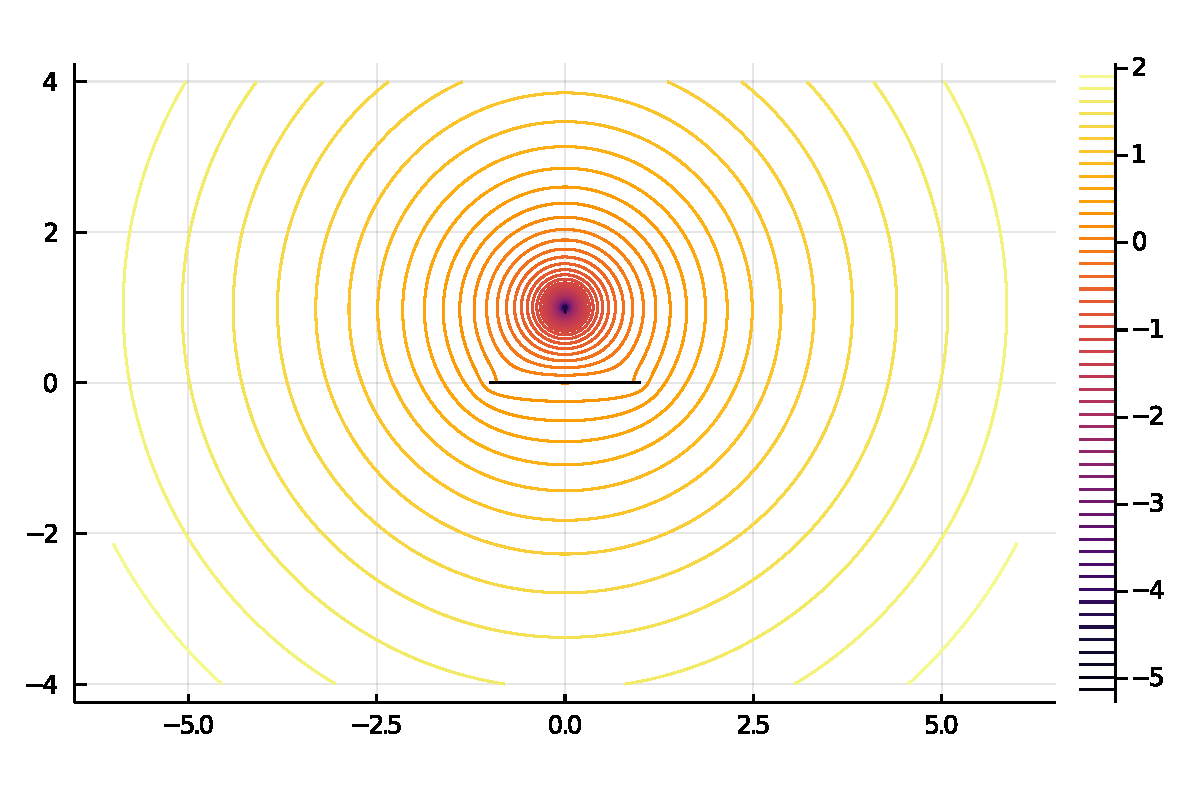
\includegraphics[width=\linewidth]{C:/Users/mfaso/OneDrive/Documents/GitHub/M3M6AppliedComplexAnalysis/output/figures/Solutions4_9_1.pdf}

\subsubsection{Problem 2.3}
As usual for logarithmic singular integral equations we want to solve

\[
{1 \over \pi} \dashint_{-1}^1 {u(t)  \over x-t} \dt = {f'(x)  \over \pi}
\]
we need to be a bit careful differentiating $f$:

\[
{\D \over \dx} \log|x-\I| = {\D \over \dx} \log\sqrt{x^2 + 1} = { x \over x^2 + 1}
\]
Now we do our usual game and solve for $u$ using the inverse Hilbert transform formula. That is, first calculate

\[
C[\sqrt{1-x^2} {x \over x^2+1}](z) = {z \sqrt{z-1} \sqrt{z+1} \over 2\I (z^2+1)} - {1 \over 2 \I} + {\I \sqrt{\I - 1} \sqrt{\I+1} \over 4 (z-\I)} +  {\I \sqrt{-\I - 1} \sqrt{-\I+1} \over 4 (z+\I)}
\]
Therefore, we know that

\[
u(x) =  -{\sqrt{\I - 1} \sqrt{\I+1} \over 2 \pi (x-\I)\sqrt{1-x^2}} -  {\sqrt{-\I - 1} \sqrt{-\I+1} \over 2 \pi (x+\I) \sqrt{1-x^2}} + {C \over \sqrt{1-x^2}}
\]
We can show (e.g. by finding its Cauchy transform and looking at the asymptotic behaviour) that

\[
\int_{-1}^1\left[- {\sqrt{\I - 1} \sqrt{\I+1} \over 2 \pi (x-\I)\sqrt{1-x^2}} -  {\sqrt{-\I - 1} \sqrt{-\I+1} \over 2 \pi (x+\I) \sqrt{1-x^2}} \right]\dx = 1
\]
Combined with the fact that

\[
\int_{-1}^1 {1 \over \sqrt{1-x^2}} = \pi
\]
we find that $C = -1/\pi$.

\emph{Verification} Let's check our work. First we see that the Hilbert transform of $u$ does indeed satisfy the specified equation (using the numerical \texttt{u} as calculated above):


\begin{lstlisting}
(*@\HLJLn{fp}@*) (*@\HLJLoB{=}@*) (*@\HLJLn{x}@*) (*@\HLJLoB{->}@*) (*@\HLJLoB{-}@*)(*@\HLJLn{x}@*)(*@\HLJLoB{/}@*)(*@\HLJLp{(}@*)(*@\HLJLn{x}@*)(*@\HLJLoB{{\textasciicircum}}@*)(*@\HLJLni{2}@*)(*@\HLJLoB{+}@*)(*@\HLJLni{1}@*)(*@\HLJLp{)}@*)
(*@\HLJLcs{{\#}}@*) (*@\HLJLcs{note}@*) (*@\HLJLcs{that}@*) (*@\HLJLcs{the}@*) (*@\HLJLcs{numerically}@*) (*@\HLJLcs{calculated}@*) (*@\HLJLcs{u}@*) (*@\HLJLcs{is}@*) (*@\HLJLcs{the}@*) (*@\HLJLcs{negative}@*) (*@\HLJLcs{of}@*) (*@\HLJLcs{the}@*) (*@\HLJLcs{solution}@*)
(*@\HLJLcs{{\#}}@*) (*@\HLJLcs{we}@*) (*@\HLJLcs{calculated}@*) (*@\HLJLcs{since}@*) (*@\HLJLcs{it}@*) (*@\HLJLcs{satisfies}@*) (*@\HLJLcs{H(u)}@*) (*@\HLJLcs{=}@*) (*@\HLJLcs{-f{\textquotesingle}/\ensuremath{\pi}}@*)
(*@\HLJLnf{H}@*)(*@\HLJLp{(}@*)(*@\HLJLn{u}@*)(*@\HLJLp{,}@*) (*@\HLJLnfB{0.1}@*)(*@\HLJLp{)}@*) (*@\HLJLp{,}@*) (*@\HLJLnf{fp}@*)(*@\HLJLp{(}@*)(*@\HLJLnfB{0.1}@*)(*@\HLJLp{)}@*)(*@\HLJLoB{/}@*)(*@\HLJLn{\ensuremath{\pi}}@*)
\end{lstlisting}

\begin{lstlisting}
(-0.03151583031523278, -0.031515830315226805)
\end{lstlisting}


And the Cauchy transform of $\sqrt{1-x^2} f'(x)$ satisfies the derived formula:


\begin{lstlisting}
(*@\HLJLn{Cf}@*) (*@\HLJLoB{=}@*) (*@\HLJLn{z}@*) (*@\HLJLoB{->}@*) (*@\HLJLn{z}@*) (*@\HLJLoB{*}@*) (*@\HLJLnf{sqrt}@*)(*@\HLJLp{(}@*)(*@\HLJLn{z}@*)(*@\HLJLoB{-}@*)(*@\HLJLni{1}@*)(*@\HLJLp{)}@*)(*@\HLJLnf{sqrt}@*)(*@\HLJLp{(}@*)(*@\HLJLn{z}@*)(*@\HLJLoB{+}@*)(*@\HLJLni{1}@*)(*@\HLJLp{)}@*)(*@\HLJLoB{/}@*)(*@\HLJLp{(}@*)(*@\HLJLni{2}@*)(*@\HLJLn{im}@*)(*@\HLJLoB{*}@*)(*@\HLJLp{(}@*)(*@\HLJLn{z}@*)(*@\HLJLoB{{\textasciicircum}}@*)(*@\HLJLni{2}@*)(*@\HLJLoB{+}@*)(*@\HLJLni{1}@*)(*@\HLJLp{))}@*) (*@\HLJLoB{-}@*) (*@\HLJLni{1}@*)(*@\HLJLoB{/}@*)(*@\HLJLp{(}@*)(*@\HLJLni{2}@*)(*@\HLJLn{im}@*)(*@\HLJLp{)}@*) (*@\HLJLoB{+}@*) (*@\HLJLn{im}@*)(*@\HLJLoB{*}@*)(*@\HLJLnf{sqrt}@*)(*@\HLJLp{(}@*)(*@\HLJLn{im}@*)(*@\HLJLoB{-}@*)(*@\HLJLni{1}@*)(*@\HLJLp{)}@*)(*@\HLJLnf{sqrt}@*)(*@\HLJLp{(}@*)(*@\HLJLn{im}@*)(*@\HLJLoB{+}@*)(*@\HLJLni{1}@*)(*@\HLJLp{)}@*)(*@\HLJLoB{/}@*)(*@\HLJLp{(}@*)(*@\HLJLni{4}@*)(*@\HLJLp{(}@*)(*@\HLJLn{z}@*)(*@\HLJLoB{-}@*)(*@\HLJLn{im}@*)(*@\HLJLp{))}@*) (*@\HLJLoB{+}@*)
         (*@\HLJLn{im}@*)(*@\HLJLoB{*}@*)(*@\HLJLnf{sqrt}@*)(*@\HLJLp{(}@*)(*@\HLJLoB{-}@*)(*@\HLJLn{im}@*)(*@\HLJLoB{-}@*)(*@\HLJLni{1}@*)(*@\HLJLp{)}@*)(*@\HLJLnf{sqrt}@*)(*@\HLJLp{(}@*)(*@\HLJLoB{-}@*)(*@\HLJLn{im}@*)(*@\HLJLoB{+}@*)(*@\HLJLni{1}@*)(*@\HLJLp{)}@*)(*@\HLJLoB{/}@*)(*@\HLJLp{(}@*)(*@\HLJLni{4}@*)(*@\HLJLp{(}@*)(*@\HLJLn{z}@*)(*@\HLJLoB{+}@*)(*@\HLJLn{im}@*)(*@\HLJLp{))}@*)
(*@\HLJLoB{-}@*)(*@\HLJLnf{cauchy}@*)(*@\HLJLp{(}@*)(*@\HLJLnf{sqrt}@*)(*@\HLJLp{(}@*)(*@\HLJLni{1}@*)(*@\HLJLoB{-}@*)(*@\HLJLn{x}@*)(*@\HLJLoB{{\textasciicircum}}@*)(*@\HLJLni{2}@*)(*@\HLJLp{)}@*)(*@\HLJLnf{fp}@*)(*@\HLJLp{(}@*)(*@\HLJLn{x}@*)(*@\HLJLp{),}@*) (*@\HLJLn{z}@*)(*@\HLJLp{)}@*) (*@\HLJLp{,}@*) (*@\HLJLnf{Cf}@*)(*@\HLJLp{(}@*)(*@\HLJLn{z}@*)(*@\HLJLp{)}@*)
\end{lstlisting}

\begin{lstlisting}
(0.02014804460385935 - 0.004468734515943387im, 0.02014804460385937 - 0.0044
68734515943457im)
\end{lstlisting}


Therefore we can invert to the Hilbert transform for $f'$:


\begin{lstlisting}
(*@\HLJLn{w}@*) (*@\HLJLoB{=}@*) (*@\HLJLoB{-}@*)(*@\HLJLnf{H}@*)(*@\HLJLp{(}@*)(*@\HLJLnf{sqrt}@*)(*@\HLJLp{(}@*)(*@\HLJLni{1}@*)(*@\HLJLoB{-}@*)(*@\HLJLn{x}@*)(*@\HLJLoB{{\textasciicircum}}@*)(*@\HLJLni{2}@*)(*@\HLJLp{)}@*)(*@\HLJLnf{fp}@*)(*@\HLJLp{(}@*)(*@\HLJLn{x}@*)(*@\HLJLp{))}@*)(*@\HLJLoB{/}@*)(*@\HLJLnf{sqrt}@*)(*@\HLJLp{(}@*)(*@\HLJLni{1}@*)(*@\HLJLoB{-}@*)(*@\HLJLn{x}@*)(*@\HLJLoB{{\textasciicircum}}@*)(*@\HLJLni{2}@*)(*@\HLJLp{)}@*)
(*@\HLJLn{w2}@*) (*@\HLJLoB{=}@*) (*@\HLJLnf{sqrt}@*)(*@\HLJLp{(}@*)(*@\HLJLn{im}@*)(*@\HLJLoB{-}@*)(*@\HLJLni{1}@*)(*@\HLJLp{)}@*)(*@\HLJLnf{sqrt}@*)(*@\HLJLp{(}@*)(*@\HLJLn{im}@*)(*@\HLJLoB{+}@*)(*@\HLJLni{1}@*)(*@\HLJLp{)}@*)(*@\HLJLoB{/}@*)(*@\HLJLp{(}@*)(*@\HLJLni{2}@*)(*@\HLJLp{(}@*)(*@\HLJLn{x}@*)(*@\HLJLoB{-}@*)(*@\HLJLn{im}@*)(*@\HLJLp{)}@*) (*@\HLJLoB{*}@*) (*@\HLJLnf{sqrt}@*)(*@\HLJLp{(}@*)(*@\HLJLni{1}@*)(*@\HLJLoB{-}@*)(*@\HLJLn{x}@*)(*@\HLJLoB{{\textasciicircum}}@*)(*@\HLJLni{2}@*)(*@\HLJLp{))}@*) (*@\HLJLoB{+}@*)
         (*@\HLJLnf{sqrt}@*)(*@\HLJLp{(}@*)(*@\HLJLoB{-}@*)(*@\HLJLn{im}@*)(*@\HLJLoB{-}@*)(*@\HLJLni{1}@*)(*@\HLJLp{)}@*)(*@\HLJLnf{sqrt}@*)(*@\HLJLp{(}@*)(*@\HLJLoB{-}@*)(*@\HLJLn{im}@*)(*@\HLJLoB{+}@*)(*@\HLJLni{1}@*)(*@\HLJLp{)}@*)(*@\HLJLoB{/}@*)(*@\HLJLp{(}@*)(*@\HLJLni{2}@*)(*@\HLJLp{(}@*)(*@\HLJLn{x}@*)(*@\HLJLoB{+}@*)(*@\HLJLn{im}@*)(*@\HLJLp{)}@*) (*@\HLJLoB{*}@*) (*@\HLJLnf{sqrt}@*)(*@\HLJLp{(}@*)(*@\HLJLni{1}@*)(*@\HLJLoB{-}@*)(*@\HLJLn{x}@*)(*@\HLJLoB{{\textasciicircum}}@*)(*@\HLJLni{2}@*)(*@\HLJLp{))}@*)
(*@\HLJLnf{H}@*)(*@\HLJLp{(}@*)(*@\HLJLn{w}@*)(*@\HLJLp{,}@*)(*@\HLJLnfB{0.1}@*)(*@\HLJLp{)}@*) (*@\HLJLp{,}@*) (*@\HLJLnf{H}@*)(*@\HLJLp{(}@*)(*@\HLJLn{w2}@*)(*@\HLJLp{,}@*)(*@\HLJLnfB{0.1}@*)(*@\HLJLp{)}@*) (*@\HLJLp{,}@*) (*@\HLJLnf{fp}@*)(*@\HLJLp{(}@*)(*@\HLJLnfB{0.1}@*)(*@\HLJLp{)}@*)
\end{lstlisting}

\begin{lstlisting}
(-0.09900990099009971, -0.09900990099010008 - 0.0im, -0.09900990099009901)
\end{lstlisting}


And we have recovered $u$ up to $C/\sqrt{1-x^2}$:


\begin{lstlisting}
(*@\HLJLn{C}@*) (*@\HLJLoB{=}@*) (*@\HLJLoB{-}@*)(*@\HLJLni{1}@*)(*@\HLJLoB{/}@*)(*@\HLJLn{\ensuremath{\pi}}@*)

(*@\HLJLoB{-}@*)(*@\HLJLnf{u}@*)(*@\HLJLp{(}@*)(*@\HLJLnfB{0.1}@*)(*@\HLJLp{)}@*) (*@\HLJLp{,}@*) (*@\HLJLoB{-}@*)(*@\HLJLnf{w2}@*)(*@\HLJLp{(}@*)(*@\HLJLnfB{0.1}@*)(*@\HLJLp{)}@*)(*@\HLJLoB{/}@*)(*@\HLJLn{\ensuremath{\pi}}@*) (*@\HLJLoB{+}@*) (*@\HLJLn{C}@*)(*@\HLJLoB{/}@*)(*@\HLJLnf{sqrt}@*)(*@\HLJLp{(}@*)(*@\HLJLni{1}@*)(*@\HLJLoB{-}@*)(*@\HLJLnfB{0.1}@*)(*@\HLJLoB{{\textasciicircum}}@*)(*@\HLJLni{2}@*)(*@\HLJLp{)}@*)
\end{lstlisting}

\begin{lstlisting}
(0.1280330340643996, 0.12803303406431615 - 0.0im)
\end{lstlisting}


\subsection{Problem 3}
\subsubsection{Problem 3.1}
We actually start by showing the second properties of Problem 3.2, for all $\alpha$:


\begin{align*}
{\D \over \dx} \br[x^\alpha \E^{-x} L_n^{(\alpha)}(x)] &= {1 \over n!}  {\D^{n+1} \over \dx^{n+1}}\br[x^{\alpha+n}\E^{-x}] \ccr
= (n+1)x^{\alpha-1}\E^{-x}  {x^{1-\alpha} \E^{x} \over (n+1)!}{ \D^{n+1} \over \dx^{n+1}}\br[x^{\alpha+n}\E^{-x}] \ccr
= (n+1) x^{\alpha-1}\E^{-x} L_{n+1}^{(\alpha-1)}(x).
\end{align*}
Expanding out the derivative we see

\[
x^{\alpha-1} \E^{-x}\pr({(\alpha -x)L_n^{(\alpha)}(x) + (L_n^{(\alpha)})'(x)}) = (n+1) x^{\alpha-1}\E^{-x} L_{n+1}^{(\alpha-1)}(x)
\]
or in other words

\[
(\alpha -x)L_n^{(\alpha)}(x) + (L_n^{(\alpha)})'(x) = (n+1) L_{n+1}^{(\alpha-1)}(x)
\]
By induction with the fact $L_0^{(\alpha)}(x) = 1$, we therefore get

\[
L_n^{(\alpha)}(x) = {(\alpha+1 -x)L_{n-1}^{(\alpha+1)}(x) + (L_n^{(\alpha+1)})'(x) \over n}
\]
is a degree $n$ polynomial. We further have that the leading coefficient is


\begin{align*}
L_n^{(\alpha)}(x) &= -{x \over n} L_{n-1}^{(\alpha+1)}(x) +O(x^{n-1}) =   {x^2 \over n(n-1)} L_{n-2}^{(\alpha+2)}(x) +O(x^{n-1}) = \cdots \ccr
= {(-1)^n x^n \over n!} L_0^{(\alpha+n)}(x) +O(x^{n-1}) \\
&= {(-1)^n x^n \over n!} +O(x^{n-1})
\end{align*}
We now show orthogonality with lower degree polynomials using integration by parts:

\[
\int_0^\infty L_n^{(\alpha)}(x) p_m(x) x^\alpha \E^{-x} \dx =
\int_0^\infty  {1 \over n!} {\D^n \over \dx^n}\br[x^{\alpha+n}\E^{-x}]  p_m(x)  \dx = (-1)^n \int_0^\infty  {1 \over n!} \br[x^{\alpha+n}\E^{-x}]  p_m^{(n)}(x)  \dx = 0
\]
since $p_m^{(n)}(x) = 0$. Note we use the fact that

\[
{\D^k \over \dx^k}\br[x^{\alpha+n}\E^{-x}]
\]
vanishes at zero to ignore the boundary terms in integration by parts.

\subsubsection{Problem 3.2}
We showed the second property as part of 3.1. For the first part, it is clear that we have the correct constant. Now we show orthogonality with all degree $m < n-1$ polynomials (using the fact that $x^{\alpha+1} \E^{-x}$ is zero at $x = 0$):

\[
\int_0^\infty {\D L_n^{(\alpha)}(x) \over \dx} p_m(x) x^{\alpha+1} \E^{-x} \dx = -\int_0^\infty L_n^{(\alpha)}(x) (x p_m'(x) + (\alpha+1) p_m - x p_m) x^{\alpha} \E^{-x} \dx = 0
\]
since $(x p_m'(x) + (\alpha+1) p_m - x p_m) $ is degree $m+1 < n$.

For the third part, use the product rule on the last derivative:


\begin{align*}
(n+1) L_{n+1}^{(\alpha)}(x) &= {x^{-\alpha}\E^x \over n!} {\D^{n} \over \dx^{n}} {\D \over \dx} \br[x^{\alpha+n+1} \E^{-x}] \\
  &= {x^{-\alpha}\E^x \over n!} {\D^{n} \over \dx^{n}}  \br[(\alpha+n+1)x^{\alpha+n} \E^{-x}-x^{\alpha+n+1} \E^{-x}]  \\
    &= (\alpha+n+1)L_n^{(\alpha)}(x) -   xL_n^{(\alpha+1)}(x)
\end{align*}
For the last result, we apply the product rule $n$ times:


\begin{align*}
L_{n}^{(\alpha+1)}(x) &= {x^{-1-\alpha}\E^x \over n!} {\D^{n-1} \over \dx^{n-1}} {\D \over \dx} \br[x x^{\alpha+n} \E^{-x}] \\
&= {x^{-1-\alpha}\E^x \over n!} {\D^{n-1} \over \dx^{n-1}} \br[ x^{\alpha+n} \E^{-x}]  + {x^{-1-\alpha}\E^x \over n!} {\D^{n-1} \over \dx^{n-1}} x {\D \over \dx} \br[ x^{\alpha+n} \E^{-x}]  \\
&= {2 \over n}L_{n-1}^{(\alpha+1)}(x)   + {x^{-1-\alpha}\E^x \over n!} {\D^{n-2} \over \dx^{n-2}} x {\D^2 \over \dx^2} \br[ x^{\alpha+n} \E^{-x}]  \\
&= {3 \over n}L_{n-1}^{(\alpha+1)}(x)   + {x^{-1-\alpha}\E^x \over n!} {\D^{n-3} \over \dx^{n-3}} x {\D^3 \over \dx^3} \br[ x^{\alpha+n} \E^{-x}]  \\
&\vdots\\
&={n \over n}L_{n-1}^{(\alpha+1)}(x)   + {x^{-\alpha}\E^x \over n!} {\D^{n} \over \dx^{n}}  \br[ x^{\alpha+n} \E^{-x}] \\
&=L_{n-1}^{(\alpha+1)}(x) + L_n^{(\alpha)}(x)
\end{align*}
\newpage
\subsubsection{Problem 3.3}
Note that relationship 3 above did not depend on $\alpha >-1$.  We therefore have from 3.2, comibing property (3) and (4),


\begin{align*}
x L_n^{(\alpha)}(x) &= -(n+1)L_{n+1}^{(\alpha-1)}(x) +(n+\alpha)L_n^{(\alpha-1)}(x) \\
  &= -(n+1)L_{n+1}^{(\alpha)}(x) + (n+1)L_{n}^{(\alpha)}(x) +(n+\alpha)L_{n}^{(\alpha)}(x) - (n+\alpha)L_{n-1}^{(\alpha)}(x) \\
  &= - (n+\alpha)L_{n-1}^{(\alpha)}(x) + (2n+\alpha+1) L_n^{(\alpha)}(x) -(n+1)L_{n+1}^{(\alpha)}(x)
\end{align*}
The Jacobi operator therefore has the form

\[
x \begin{pmatrix} L_0^{(\alpha)}(x) \\
            L_1^{(\alpha)}(x) \\
                \vdots
                \end{pmatrix} = \begin{pmatrix} \alpha+1 &-1 \\
                                                -1-\alpha & \alpha+3 & -2 \\
                                                   & -2-\alpha & \alpha+5 &-3 \\                  &       & -3-\alpha & \alpha+7 &-4 \\
                                                      &&   & -4-\alpha & \alpha+9 &\ddots \\
                                                      &&&&\ddots & \ddots
                                                    \end{pmatrix} \begin{pmatrix} L_0^{(\alpha)}(x) \\
            L_1^{(\alpha)}(x) \\
                \vdots
                \end{pmatrix}
\]
\subsection{Problem 4}
\subsubsection{Problem 4.1}
Note that

\[
{\D \over \dx} \E^{-x/2} u(x) =  \E^{-x/2} (-{u(x) \over 2} +u'(x))
\]
Thus
\[
{\D \over \dx} \E^{-x/2} u(x)  = \E^{-x/2} (u'(x) -{u(x) \over 2} - x u(x))
\]
\newpage

We have the derivative operator from $L_k(x)$ to $L_k^{(1)}(x)$ as:

\[
D = \begin{pmatrix}
0 & -1 \\
  &&-1 \\
  &&&\ddots
\end{pmatrix}
\]
and the Multiplication operator for $\alpha = 0$ (from Problem 3.3)

\[
J^\top = \begin{pmatrix} 1 &-1\\
                        -1 & 3 &-2\\
                            &\ddots & \ddots & \ddots
                            \end{pmatrix}
\]
and the conversion operator (from Problem 3.2 property 4)

\[
S = \begin{pmatrix}
        1 & -1 \\ & 1 & -1 \\&&\ddots & \ddots
\end{pmatrix}
\]
We thus have multiplication by $x$ from basis to the other as

\[
S J^\top = \begin{pmatrix}
2 & -4 & 2 \\
-1 & 5 & -7 & 3 \\
& -2 & 8 & -10 & 4\\
&&\ddots&\ddots&\ddots&\ddots
\end{pmatrix}
\]
Putting everything together, we get the operator


\begin{lstlisting}
(*@\HLJLn{D}@*) (*@\HLJLoB{=}@*) (*@\HLJLnf{Derivative}@*)(*@\HLJLp{()}@*) (*@\HLJLoB{:}@*)  (*@\HLJLnf{Laguerre}@*)(*@\HLJLp{(}@*)(*@\HLJLni{0}@*)(*@\HLJLp{)}@*) (*@\HLJLoB{\ensuremath{\rightarrow}}@*) (*@\HLJLnf{Laguerre}@*)(*@\HLJLp{(}@*)(*@\HLJLni{1}@*)(*@\HLJLp{)}@*)
(*@\HLJLn{S}@*) (*@\HLJLoB{=}@*) (*@\HLJLn{I}@*) (*@\HLJLoB{:}@*) (*@\HLJLnf{Laguerre}@*)(*@\HLJLp{(}@*)(*@\HLJLni{0}@*)(*@\HLJLp{)}@*) (*@\HLJLoB{\ensuremath{\rightarrow}}@*) (*@\HLJLnf{Laguerre}@*)(*@\HLJLp{(}@*)(*@\HLJLni{1}@*)(*@\HLJLp{)}@*)

(*@\HLJLn{Jt}@*) (*@\HLJLoB{=}@*) (*@\HLJLnf{Recurrence}@*)(*@\HLJLp{(}@*)(*@\HLJLnf{Laguerre}@*)(*@\HLJLp{(}@*)(*@\HLJLni{0}@*)(*@\HLJLp{))}@*)

(*@\HLJLp{(}@*)(*@\HLJLn{D}@*) (*@\HLJLoB{-}@*) (*@\HLJLn{S}@*)(*@\HLJLoB{/}@*)(*@\HLJLni{2}@*) (*@\HLJLoB{-}@*)(*@\HLJLn{S}@*)(*@\HLJLoB{*}@*)(*@\HLJLn{Jt}@*)(*@\HLJLp{)[}@*)(*@\HLJLni{1}@*)(*@\HLJLoB{:}@*)(*@\HLJLni{10}@*)(*@\HLJLp{,}@*)(*@\HLJLni{1}@*)(*@\HLJLoB{:}@*)(*@\HLJLni{10}@*)(*@\HLJLp{]}@*)
\end{lstlisting}

\begin{lstlisting}
10(*@\ensuremath{\times}@*(10 BandedMatrices.BandedMatrix(*@{{\{}}@*)Complex(*@{{\{}}@*)Float64(*@{{\}}}@*),Array(*@{{\{}}@*)Complex(*@{{\{}}@*)Float64(*@{{\}}}@*),2
(*@{{\}}}@*),Base.OneTo(*@{{\{}}@*)Int64(*@{{\}}}@*)(*@{{\}}}@*):
 -2.5+0.0im   3.5+0.0im  -2.0+0.0im        (*@\ensuremath{\cdot}@*(      (*@\ensuremath{\ldots}@*(        (*@\ensuremath{\cdot}@*(            (*@\ensuremath{\cdot}@*(  
  
  1.0+0.0im  -5.5+0.0im   6.5+0.0im   -3.0+0.0im           (*@\ensuremath{\cdot}@*(            (*@\ensuremath{\cdot}@*(  
  
      (*@\ensuremath{\cdot}@*(       2.0+0.0im  -8.5+0.0im    9.5+0.0im           (*@\ensuremath{\cdot}@*(            (*@\ensuremath{\cdot}@*(  
  
      (*@\ensuremath{\cdot}@*(           (*@\ensuremath{\cdot}@*(       3.0+0.0im  -11.5+0.0im           (*@\ensuremath{\cdot}@*(            (*@\ensuremath{\cdot}@*(  
  
      (*@\ensuremath{\cdot}@*(           (*@\ensuremath{\cdot}@*(           (*@\ensuremath{\cdot}@*(        4.0+0.0im           (*@\ensuremath{\cdot}@*(            (*@\ensuremath{\cdot}@*(  
  
      (*@\ensuremath{\cdot}@*(           (*@\ensuremath{\cdot}@*(           (*@\ensuremath{\cdot}@*(            (*@\ensuremath{\cdot}@*(      (*@\ensuremath{\ldots}@*(        (*@\ensuremath{\cdot}@*(            (*@\ensuremath{\cdot}@*(  
  
      (*@\ensuremath{\cdot}@*(           (*@\ensuremath{\cdot}@*(           (*@\ensuremath{\cdot}@*(            (*@\ensuremath{\cdot}@*(          -8.0+0.0im        (*@\ensuremath{\cdot}@*(  
  
      (*@\ensuremath{\cdot}@*(           (*@\ensuremath{\cdot}@*(           (*@\ensuremath{\cdot}@*(            (*@\ensuremath{\cdot}@*(          24.5+0.0im   -9.0+0.0
im
      (*@\ensuremath{\cdot}@*(           (*@\ensuremath{\cdot}@*(           (*@\ensuremath{\cdot}@*(            (*@\ensuremath{\cdot}@*(         -26.5+0.0im   27.5+0.0
im
      (*@\ensuremath{\cdot}@*(           (*@\ensuremath{\cdot}@*(           (*@\ensuremath{\cdot}@*(            (*@\ensuremath{\cdot}@*(           9.0+0.0im  -29.5+0.0
im
\end{lstlisting}


\subsubsection{Problem 4.2}
We have


\begin{align*}
{\E^x \over x^\alpha} {\D \over \dx} \br[x^{\alpha+1} \E^{-x} {\D L_n^{(\alpha)} \over \dx}] &= -{\E^x \over x^\alpha} {\D \over \dx} \br[x^{\alpha+1} \E^{-x} { L_{n-1}^{(\alpha+1)} \over \dx}] \\
&= -n L_{n}^{(\alpha)}(x)
\end{align*}
Therefore $\lambda_n = -n$. This can be expanded in the form:

\[
x {\D^2 L_n^{(\alpha)} \over \dx^2} + (\alpha+1 - x) {\D L_n^{(\alpha)} \over \dx} = -n L_n^{(\alpha)}(x)
\]

}
\end{document}
